\cleardoublepage

\chapter{Estado de la cuestión}
\label{makereference2}

% - estado inicial con la herramienta original que no funcionaba?

Contextualizando el entorno, la transición hacia un sistema energético descarbonizado, impulsada por la creciente penetración de fuentes de energía renovable, como la solar fotovoltaica y la eólica, presenta desafíos significativos para la estabilidad y gestión de la red eléctrica~\cite{carrasco2023battery}. De esta forma, los \gls{bess} emergen como una tecnología clave para dotar de flexibilidad al sistema, solucionando el desacoplo entre la generación y el consumo de electricidad~\cite{gissey2018market}.

El mercado eléctrico, que opera usando un modelo marginalista para los mercados spot en donde el precio es determinado mediante el cruze de la oferta y demanda mostrado en la figura~\ref{fig:precio-casacion}, ofrece diversas oportunidades para los \glspl{bess}. Estas incluyen el arbitraje de energía en los mercados spot diario intradiarios y continuo, en los que se centra el sistema desarrollado, y la participación en los servicios de ajuste~\cite{gaspar2021optimisation}, \gls{afrr} y \gls{mfrr}, donde se arbitran disponibilidades. Por ello, la viabilidad económica depende intrínsecamente de la capacidad del sistema para formular y ejecutar estrategias de operación óptimas en un entorno de alta incertidumbre de precios y previsiones de generación~\cite{heredia2015economic}, llamandola incluso una ``tecnología clave''.

\begin{figure}
  \centering
  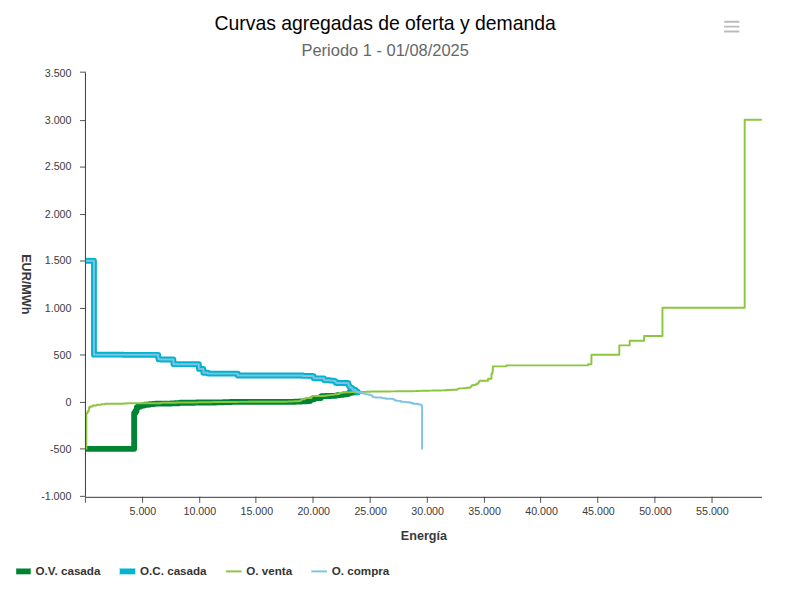
\includegraphics[width=0.5\linewidth]{figures/precio-casacion.png}
  \caption{Curva de casación real del inicio del mes de agosto del mercado eléctrico marginalista extraída de \gls{omie}, donde tan solo las ofertas de compra por encima y de venta por debajo del precio de casación son aceptadas}
  \label{fig:precio-casacion}
\end{figure}

\section{Situación tecnológica}

La situación tecnológica de los optimizadores de \glspl{bess} varía significativamente entre los mercados eléctricos ibéricos, del resto de Europa y de Estados Unidos, debido a diferencias en el diseño de los mercados, los marcos regulatorios y los incentivos políticos.
